% This file is generated by the MATLAB m-file laprint.m. It can be included
% into LaTeX documents using the packages graphicx, color and psfrag.
% It is accompanied by a postscript file. A sample LaTeX file is:
%    \documentclass{article}\usepackage{graphicx,color,psfrag}
%    \begin{document}% This file is generated by the MATLAB m-file laprint.m. It can be included
% into LaTeX documents using the packages graphicx, color and psfrag.
% It is accompanied by a postscript file. A sample LaTeX file is:
%    \documentclass{article}\usepackage{graphicx,color,psfrag}
%    \begin{document}% This file is generated by the MATLAB m-file laprint.m. It can be included
% into LaTeX documents using the packages graphicx, color and psfrag.
% It is accompanied by a postscript file. A sample LaTeX file is:
%    \documentclass{article}\usepackage{graphicx,color,psfrag}
%    \begin{document}% This file is generated by the MATLAB m-file laprint.m. It can be included
% into LaTeX documents using the packages graphicx, color and psfrag.
% It is accompanied by a postscript file. A sample LaTeX file is:
%    \documentclass{article}\usepackage{graphicx,color,psfrag}
%    \begin{document}\input{MCMC_sigmas_rp_spin_1}\end{document}
% See http://www.mathworks.de/matlabcentral/fileexchange/loadFile.do?objectId=4638
% for recent versions of laprint.m.
%
% created by:           LaPrint version 3.16 (13.9.2004)
% created on:           08-Aug-2012 15:09:54
% eps bounding box:     15 cm x 11.25 cm
% comment:              
%
\begin{psfrags}%
\psfragscanon%
%
% text strings:
\psfrag{s05}[t][t]{\color[rgb]{0,0,0}\setlength{\tabcolsep}{0pt}\begin{tabular}{c}{\Large$r_\mathrm{p}/r_\mathrm{g}$}\end{tabular}}%
\psfrag{s06}[b][b]{\color[rgb]{0,0,0}\setlength{\tabcolsep}{0pt}\begin{tabular}{c}{\Large$\sigma_{M_\bullet}/M_\bullet$}\end{tabular}}%
\psfrag{s09}[][]{\color[rgb]{0,0,0}\setlength{\tabcolsep}{0pt}\begin{tabular}{c} \end{tabular}}%
\psfrag{s10}[][]{\color[rgb]{0,0,0}\setlength{\tabcolsep}{0pt}\begin{tabular}{c} \end{tabular}}%
\psfrag{s11}[t][t]{\color[rgb]{0,0,0}\setlength{\tabcolsep}{0pt}\begin{tabular}{c}{\Large$\left|a_\ast\right|$}\end{tabular}}%
%
% xticklabels:
\psfrag{x01}[t][t]{$1$}%
\psfrag{x02}[t][t]{$10$}%
%
% yticklabels:
\psfrag{v01}[l][l]{$0.1$}%
\psfrag{v02}[l][l]{$0.2$}%
\psfrag{v03}[l][l]{$0.3$}%
\psfrag{v04}[l][l]{$0.4$}%
\psfrag{v05}[l][l]{$0.5$}%
\psfrag{v06}[l][l]{$0.6$}%
\psfrag{v07}[l][l]{$0.7$}%
\psfrag{v08}[l][l]{$0.8$}%
\psfrag{v09}[l][l]{$0.9$}%
\psfrag{v10}[l][l]{$1.0$}%
\psfrag{v11}[r][r]{$10^{-5}$}%
\psfrag{v12}[r][r]{$10^{-4}$}%
\psfrag{v13}[r][r]{$10^{-3}$}%
\psfrag{v14}[r][r]{$10^{-2}$}%
\psfrag{v15}[r][r]{$10^{-1}$}%
\psfrag{v16}[r][r]{$10^{0}$}%
%
% Figure:
\resizebox{12cm}{!}{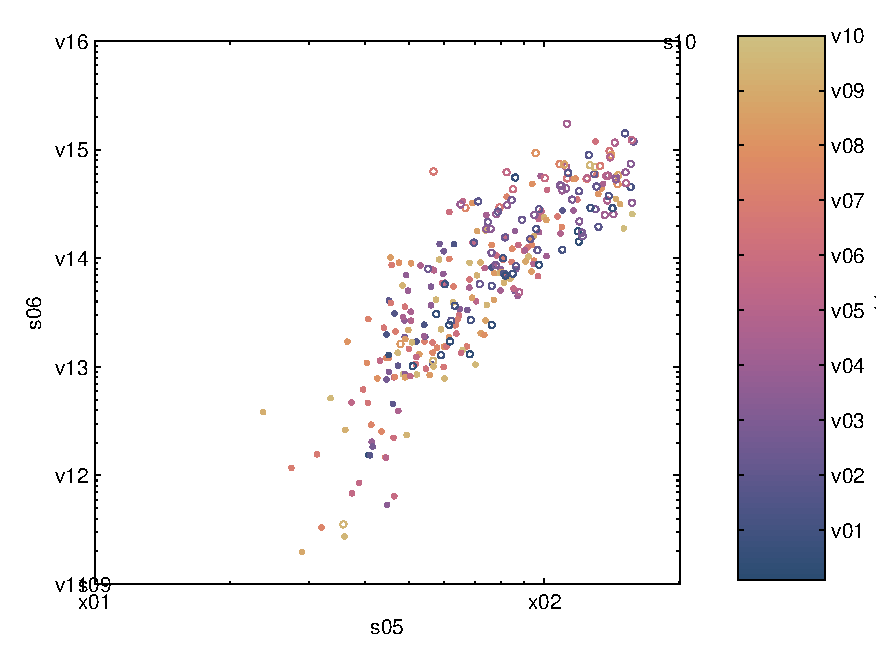
\includegraphics{MCMC_sigmas_rp_spin_1.eps}}%
\end{psfrags}%
%
% End MCMC_sigmas_rp_spin_1.tex
\end{document}
% See http://www.mathworks.de/matlabcentral/fileexchange/loadFile.do?objectId=4638
% for recent versions of laprint.m.
%
% created by:           LaPrint version 3.16 (13.9.2004)
% created on:           08-Aug-2012 15:09:54
% eps bounding box:     15 cm x 11.25 cm
% comment:              
%
\begin{psfrags}%
\psfragscanon%
%
% text strings:
\psfrag{s05}[t][t]{\color[rgb]{0,0,0}\setlength{\tabcolsep}{0pt}\begin{tabular}{c}{\Large$r_\mathrm{p}/r_\mathrm{g}$}\end{tabular}}%
\psfrag{s06}[b][b]{\color[rgb]{0,0,0}\setlength{\tabcolsep}{0pt}\begin{tabular}{c}{\Large$\sigma_{M_\bullet}/M_\bullet$}\end{tabular}}%
\psfrag{s09}[][]{\color[rgb]{0,0,0}\setlength{\tabcolsep}{0pt}\begin{tabular}{c} \end{tabular}}%
\psfrag{s10}[][]{\color[rgb]{0,0,0}\setlength{\tabcolsep}{0pt}\begin{tabular}{c} \end{tabular}}%
\psfrag{s11}[t][t]{\color[rgb]{0,0,0}\setlength{\tabcolsep}{0pt}\begin{tabular}{c}{\Large$\left|a_\ast\right|$}\end{tabular}}%
%
% xticklabels:
\psfrag{x01}[t][t]{$1$}%
\psfrag{x02}[t][t]{$10$}%
%
% yticklabels:
\psfrag{v01}[l][l]{$0.1$}%
\psfrag{v02}[l][l]{$0.2$}%
\psfrag{v03}[l][l]{$0.3$}%
\psfrag{v04}[l][l]{$0.4$}%
\psfrag{v05}[l][l]{$0.5$}%
\psfrag{v06}[l][l]{$0.6$}%
\psfrag{v07}[l][l]{$0.7$}%
\psfrag{v08}[l][l]{$0.8$}%
\psfrag{v09}[l][l]{$0.9$}%
\psfrag{v10}[l][l]{$1.0$}%
\psfrag{v11}[r][r]{$10^{-5}$}%
\psfrag{v12}[r][r]{$10^{-4}$}%
\psfrag{v13}[r][r]{$10^{-3}$}%
\psfrag{v14}[r][r]{$10^{-2}$}%
\psfrag{v15}[r][r]{$10^{-1}$}%
\psfrag{v16}[r][r]{$10^{0}$}%
%
% Figure:
\resizebox{12cm}{!}{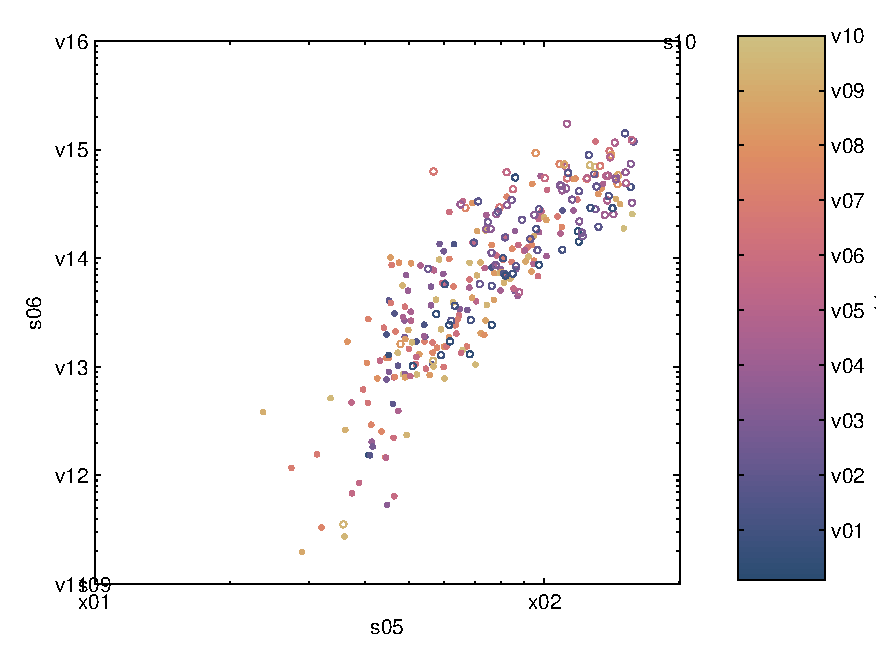
\includegraphics{MCMC_sigmas_rp_spin_1.eps}}%
\end{psfrags}%
%
% End MCMC_sigmas_rp_spin_1.tex
\end{document}
% See http://www.mathworks.de/matlabcentral/fileexchange/loadFile.do?objectId=4638
% for recent versions of laprint.m.
%
% created by:           LaPrint version 3.16 (13.9.2004)
% created on:           08-Aug-2012 15:09:54
% eps bounding box:     15 cm x 11.25 cm
% comment:              
%
\begin{psfrags}%
\psfragscanon%
%
% text strings:
\psfrag{s05}[t][t]{\color[rgb]{0,0,0}\setlength{\tabcolsep}{0pt}\begin{tabular}{c}{\Large$r_\mathrm{p}/r_\mathrm{g}$}\end{tabular}}%
\psfrag{s06}[b][b]{\color[rgb]{0,0,0}\setlength{\tabcolsep}{0pt}\begin{tabular}{c}{\Large$\sigma_{M_\bullet}/M_\bullet$}\end{tabular}}%
\psfrag{s09}[][]{\color[rgb]{0,0,0}\setlength{\tabcolsep}{0pt}\begin{tabular}{c} \end{tabular}}%
\psfrag{s10}[][]{\color[rgb]{0,0,0}\setlength{\tabcolsep}{0pt}\begin{tabular}{c} \end{tabular}}%
\psfrag{s11}[t][t]{\color[rgb]{0,0,0}\setlength{\tabcolsep}{0pt}\begin{tabular}{c}{\Large$\left|a_\ast\right|$}\end{tabular}}%
%
% xticklabels:
\psfrag{x01}[t][t]{$1$}%
\psfrag{x02}[t][t]{$10$}%
%
% yticklabels:
\psfrag{v01}[l][l]{$0.1$}%
\psfrag{v02}[l][l]{$0.2$}%
\psfrag{v03}[l][l]{$0.3$}%
\psfrag{v04}[l][l]{$0.4$}%
\psfrag{v05}[l][l]{$0.5$}%
\psfrag{v06}[l][l]{$0.6$}%
\psfrag{v07}[l][l]{$0.7$}%
\psfrag{v08}[l][l]{$0.8$}%
\psfrag{v09}[l][l]{$0.9$}%
\psfrag{v10}[l][l]{$1.0$}%
\psfrag{v11}[r][r]{$10^{-5}$}%
\psfrag{v12}[r][r]{$10^{-4}$}%
\psfrag{v13}[r][r]{$10^{-3}$}%
\psfrag{v14}[r][r]{$10^{-2}$}%
\psfrag{v15}[r][r]{$10^{-1}$}%
\psfrag{v16}[r][r]{$10^{0}$}%
%
% Figure:
\resizebox{12cm}{!}{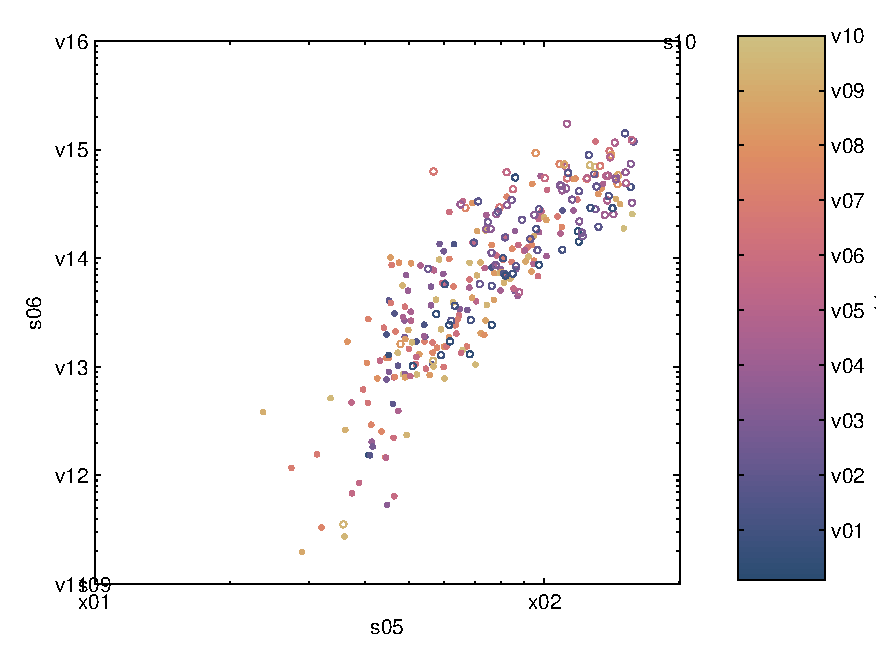
\includegraphics{MCMC_sigmas_rp_spin_1.eps}}%
\end{psfrags}%
%
% End MCMC_sigmas_rp_spin_1.tex
\end{document}
% See http://www.mathworks.de/matlabcentral/fileexchange/loadFile.do?objectId=4638
% for recent versions of laprint.m.
%
% created by:           LaPrint version 3.16 (13.9.2004)
% created on:           08-Aug-2012 15:09:54
% eps bounding box:     15 cm x 11.25 cm
% comment:              
%
\begin{psfrags}%
\psfragscanon%
%
% text strings:
\psfrag{s05}[t][t]{\color[rgb]{0,0,0}\setlength{\tabcolsep}{0pt}\begin{tabular}{c}{\Large$r_\mathrm{p}/r_\mathrm{g}$}\end{tabular}}%
\psfrag{s06}[b][b]{\color[rgb]{0,0,0}\setlength{\tabcolsep}{0pt}\begin{tabular}{c}{\Large$\sigma_{M_\bullet}/M_\bullet$}\end{tabular}}%
\psfrag{s09}[][]{\color[rgb]{0,0,0}\setlength{\tabcolsep}{0pt}\begin{tabular}{c} \end{tabular}}%
\psfrag{s10}[][]{\color[rgb]{0,0,0}\setlength{\tabcolsep}{0pt}\begin{tabular}{c} \end{tabular}}%
\psfrag{s11}[t][t]{\color[rgb]{0,0,0}\setlength{\tabcolsep}{0pt}\begin{tabular}{c}{\Large$\left|a_\ast\right|$}\end{tabular}}%
%
% xticklabels:
\psfrag{x01}[t][t]{$1$}%
\psfrag{x02}[t][t]{$10$}%
%
% yticklabels:
\psfrag{v01}[l][l]{$0.1$}%
\psfrag{v02}[l][l]{$0.2$}%
\psfrag{v03}[l][l]{$0.3$}%
\psfrag{v04}[l][l]{$0.4$}%
\psfrag{v05}[l][l]{$0.5$}%
\psfrag{v06}[l][l]{$0.6$}%
\psfrag{v07}[l][l]{$0.7$}%
\psfrag{v08}[l][l]{$0.8$}%
\psfrag{v09}[l][l]{$0.9$}%
\psfrag{v10}[l][l]{$1.0$}%
\psfrag{v11}[r][r]{$10^{-5}$}%
\psfrag{v12}[r][r]{$10^{-4}$}%
\psfrag{v13}[r][r]{$10^{-3}$}%
\psfrag{v14}[r][r]{$10^{-2}$}%
\psfrag{v15}[r][r]{$10^{-1}$}%
\psfrag{v16}[r][r]{$10^{0}$}%
%
% Figure:
\resizebox{12cm}{!}{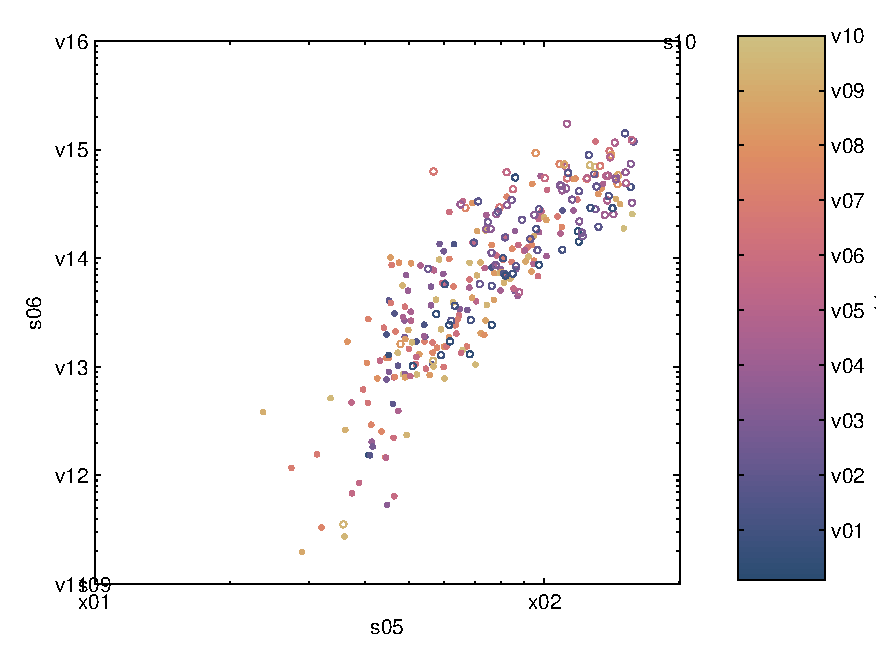
\includegraphics{MCMC_sigmas_rp_spin_1.eps}}%
\end{psfrags}%
%
% End MCMC_sigmas_rp_spin_1.tex
